\documentclass[tikz,border=10pt]{standalone}
\usepackage{amsmath}
\usepackage{amsfonts}
\usepackage{xcolor}

% Define scientific color palette
\definecolor{cpuBlue}{RGB}{230, 240, 255}
\definecolor{gpuGreen}{RGB}{235, 255, 235}
\definecolor{blockBlue}{RGB}{173, 216, 230}
\definecolor{blockGreen}{RGB}{144, 238, 144}
\definecolor{blockYellow}{RGB}{255, 255, 153}
\definecolor{blockPink}{RGB}{255, 182, 193}
\definecolor{darkGray}{RGB}{60, 60, 60}

\usetikzlibrary{shapes.geometric, arrows.meta, positioning, calc, shadows, fit}

\tikzset{
    base/.style={draw=darkGray, thick, rounded corners=2pt, align=center, font=\sffamily\small},
    proc/.style={base, fill=white, minimum width=2cm, minimum height=1cm},
    container/.style={draw=darkGray, dashed, inner sep=15pt, rounded corners=5pt},
    arrow/.style={-Stealth, thick, draw=darkGray},
    mathText/.style={font=\sffamily\scriptsize, align=center}
}

\begin{document}

% ---------------------------------------------------------------------
% DIAGRAM 1: CPU VS GPU OVERVIEW
% ---------------------------------------------------------------------
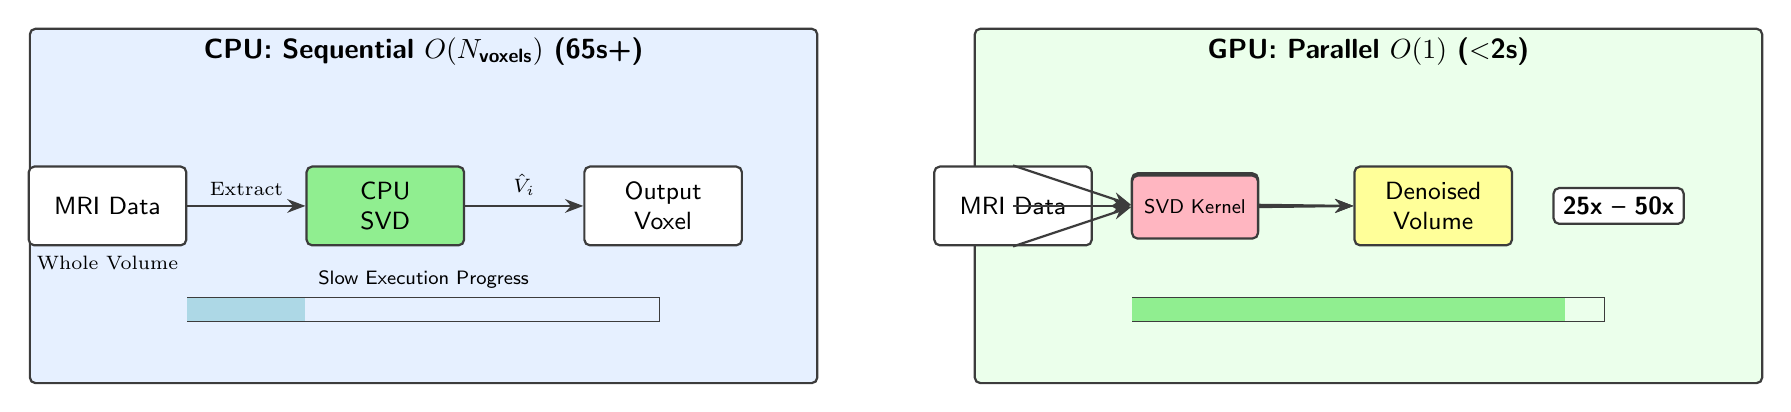
\begin{tikzpicture}
    % --- CPU SECTION ---
    \node[base, fill=cpuBlue, minimum width=10cm, minimum height=4.5cm] (cpuBox) {};
    \node[anchor=north, font=\sffamily\bfseries] at (cpuBox.north) {CPU: Sequential $O(N_{\text{voxels}})$ (65s+)};
    
    \node[proc, left=3cm of cpuBox.center, label=below:{\scriptsize Whole Volume}] (inputImg) {MRI Data};
    \node[proc, fill=blockGreen, right=1.5cm of inputImg] (cpuSvd) {CPU \\ SVD};
    \node[proc, right=1.5cm of cpuSvd] (outputVox) {Output \\ Voxel};
    
    \draw[arrow] (inputImg) -- node[above]{\scriptsize Extract} (cpuSvd);
    \draw[arrow] (cpuSvd) -- node[above]{\scriptsize $\hat{V}_i$} (outputVox);
    
    % Loading bar simulation
    \draw[darkGray, thin] ($(cpuBox.south)+(0,0.8)$) ++(-3,0) rectangle ++(6,0.3);
    \fill[blockBlue] ($(cpuBox.south)+(0,0.8)$) ++(-3,0) rectangle ++(1.5,0.3);
    \node[anchor=south, font=\sffamily\scriptsize] at ($(cpuBox.south)+(0,1.1)$) {Slow Execution Progress};

    % --- GPU SECTION ---
    \begin{scope}[xshift=12cm]
        \node[base, fill=gpuGreen, minimum width=10cm, minimum height=4.5cm] (gpuBox) {};
        \node[anchor=north, font=\sffamily\bfseries] at (gpuBox.north) {GPU: Parallel $O(1)$ ($<$2s)};
        
        \node[proc, left=3.5cm of gpuBox.center] (inputImgG) {MRI Data};
        
        % Parallel blocks
        \node[proc, fill=blockPink, right=1.5cm of inputImgG.north, yshift=-0.5cm, scale=0.8] (k1) {SVD Kernel};
        \node[proc, fill=blockPink, right=1.5cm of inputImgG.center, scale=0.8] (k2) {SVD Kernel};
        \node[proc, fill=blockPink, right=1.5cm of inputImgG.south, yshift=0.5cm, scale=0.8] (k3) {SVD Kernel};
        
        \node[proc, fill=blockYellow, right=1.2cm of k2] (assembly) {Denoised \\ Volume};
        
        \draw[arrow] (inputImgG.north) -- (k1.west);
        \draw[arrow] (inputImgG.center) -- (k2.west);
        \draw[arrow] (inputImgG.south) -- (k3.west);
        
        \draw[arrow] (k1.east) -- (assembly.west);
        \draw[arrow] (k2.east) -- (assembly.west);
        \draw[arrow] (k3.east) -- (assembly.west);
        
        % Speedup badge
        \node[base, fill=white, thick, right=0.5cm of assembly] (badge) {\bfseries 25x -- 50x};
        
        % Loading bar simulation
        \draw[darkGray, thin] ($(gpuBox.south)+(0,0.8)$) ++(-3,0) rectangle ++(6,0.3);
        \fill[blockGreen] ($(gpuBox.south)+(0,0.8)$) ++(-3,0) rectangle ++(5.5,0.3);
    \end{scope}
\end{tikzpicture}

\newpage

% ---------------------------------------------------------------------
% DIAGRAM 2: DETAILED WGPU KERNEL ARCHITECTURE
% ---------------------------------------------------------------------
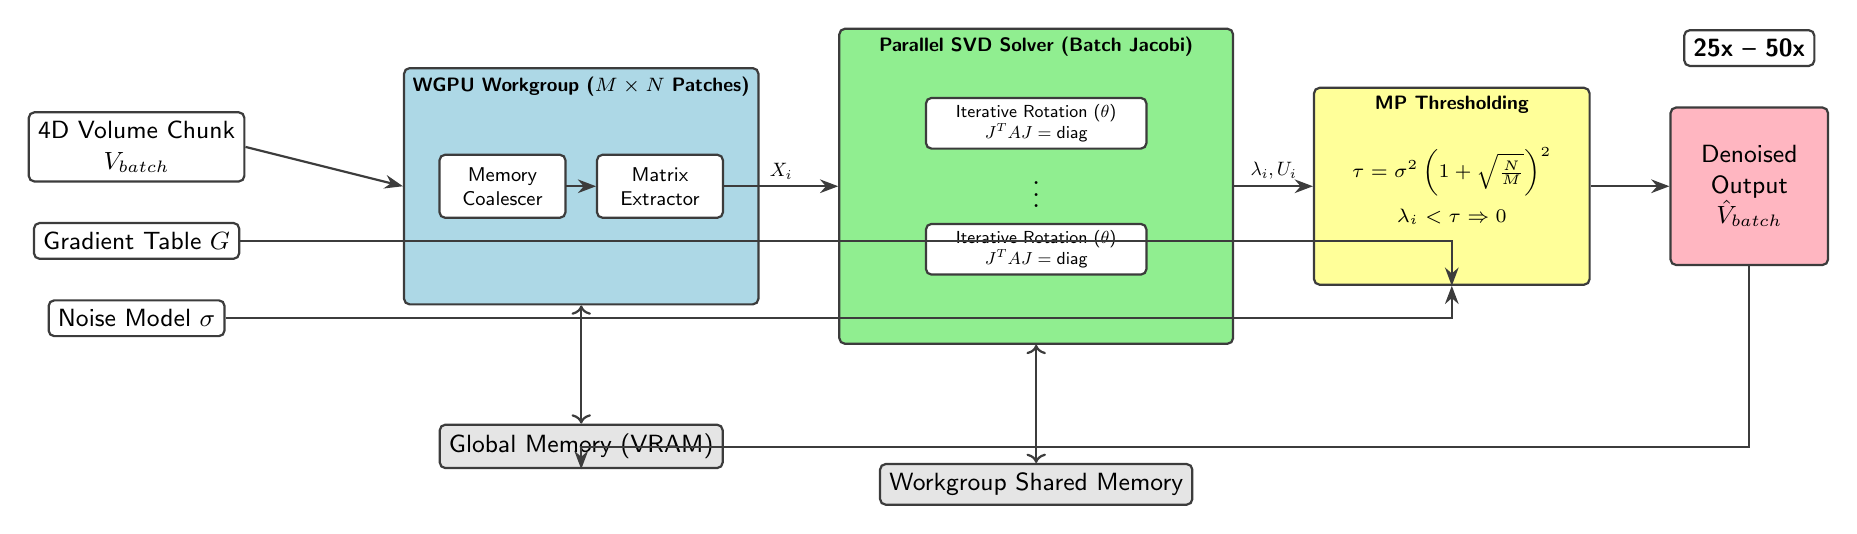
\begin{tikzpicture}[node distance=1.5cm and 2cm]

    % --- INPUTS ---
    \node[base, fill=white] (vIn) {4D Volume Chunk \\ $V_{batch}$};
    \node[base, fill=white, below=0.5cm of vIn] (gTab) {Gradient Table $G$};
    \node[base, fill=white, below=0.5cm of gTab] (noise) {Noise Model $\sigma$};

    % --- LAYER 1: WORKGROUP ---
    \node[base, fill=blockBlue, right=of vIn, minimum width=4.5cm, minimum height=3cm, yshift=-0.5cm] (workgroup) {};
    \node[anchor=north, font=\sffamily\bfseries\scriptsize] at (workgroup.north) {WGPU Workgroup ($M \times N$ Patches)};
    
    \node[proc, scale=0.8] at ($(workgroup.center)+(-1,0)$) (memC) {Memory \\ Coalescer};
    \node[proc, scale=0.8] at ($(workgroup.center)+(1,0)$) (patchEx) {Matrix \\ Extractor};
    \draw[arrow] (memC) -- (patchEx);

    % --- LAYER 2: PARALLEL SVD ---
    \node[base, fill=blockGreen, right=1cm of workgroup, minimum width=5cm, minimum height=4cm] (svdBox) {};
    \node[anchor=north, font=\sffamily\bfseries\scriptsize] at (svdBox.north) {Parallel SVD Solver (Batch Jacobi)};
    
    \node[base, fill=white, scale=0.7, minimum width=4cm] at ($(svdBox.center)+(0,0.8)$) (jac1) {Iterative Rotation ($\theta$) \\ $J^T A J = \text{diag}$};
    \node[base, fill=white, scale=0.7, minimum width=4cm] at ($(svdBox.center)+(0,-0.8)$) (jac2) {Iterative Rotation ($\theta$) \\ $J^T A J = \text{diag}$};
    \node at ($(jac1)!0.5!(jac2)$) {\vdots};

    % --- LAYER 3: THRESHOLDING ---
    \node[base, fill=blockYellow, right=1cm of svdBox, minimum width=3.5cm, minimum height=2.5cm] (threshold) {};
    \node[anchor=north, font=\sffamily\bfseries\scriptsize] at (threshold.north) {MP Thresholding};
    \node[mathText] at (threshold.center) {$\tau = \sigma^2 \left(1 + \sqrt{\frac{N}{M}}\right)^2$ \\ \\ $\lambda_i < \tau \Rightarrow 0$};

    % --- LAYER 4: ASSEMBLY ---
    \node[base, fill=blockPink, right=1cm of threshold, minimum width=2cm, minimum height=2cm] (output) {Denoised \\ Output \\ $\hat{V}_{batch}$};

    % --- GLOBAL MEMORY BLOCKS ---
    \node[base, below=1.5cm of workgroup, fill=gray!20] (globalMem) {Global Memory (VRAM)};
    \node[base, below=1.5cm of svdBox, fill=gray!20] (sharedMem) {Workgroup Shared Memory};

    % --- CONNECTIONS ---
    \draw[arrow] (vIn.east) -- (workgroup.west);
    \draw[arrow] (gTab.east) -| (threshold.south);
    \draw[arrow] (noise.east) -| (threshold.south);
    
    \draw[arrow] (patchEx.east) -- node[above, scale=0.7]{$X_i$} (svdBox.west);
    \draw[arrow] (svdBox.east) -- node[above, scale=0.7]{$\lambda_i, U_i$} (threshold.west);
    \draw[arrow] (threshold.east) -- (output.west);
    
    % Memory connections
    \draw[arrow, <->] (workgroup.south) -- (globalMem.north);
    \draw[arrow, <->] (svdBox.south) -- (sharedMem.north);
    \draw[arrow] (output.south) -- ++(0,-2.3) -| (globalMem.south);

    % Legend/Badge
    \node[base, fill=white, thick, above=0.5cm of output] (badge2) {\bfseries 25x -- 50x};

\end{tikzpicture}

\end{document}